\documentclass[a4paper, 11pt]{article}
\usepackage{fullpage}
\usepackage[german]{babel}
\usepackage{graphicx}
\usepackage{hyperref}

\begin{document}
\noindent
\large\textbf{Programmierübung 2} \\
\textbf{Bloom Filter} \\
\normalsize FHNW Brugg Windisch - Diskrete Stochastik \\
Bearbeitet von Anessollah Ima und Jonathan Bättig\hfill Datum: 25.11.2019 \\
 

\section*{A) Idee des Bloom Filters}
Der Bloom Filter ermöglicht es sehr schnell zu prüfen, ob ein Element in einer Liste vorhanden ist oder nicht. Die Berechnung erfolgt mittels Hashing unter Verwendung eines Byte Array. Mit mehreren Hash Methoden wird ein Objekt in Indexe zerlegt, welche im Bloom Filter Byte Array als belegt markiert werden. Dabei werden bereits belegte Plätze im Array ignoriert. In unserem Anwendungsfall kann der Filter der Initialisierung gefragt werden, ob ein Element vorhanden ist oder nicht. Wenn der Bloom Filter behauptet, dass ein Element noch nicht in der Liste ist, so stimmt diese Aussage immer zu 100\%. Ergibt die Berechnungen des Filters allerdings, dass das Element bereits vorhanden ist, so darf man dem Filter nicht trauen. Es ist möglich, dass das Element trotzdem noch nicht vorhanden ist. Der Bloom Filter ist nämlich eine probabilistische Datenstruktur. Er eignet sich somit primär für Szenarien, in denen geprüft werden muss, ob eine Liste oder Tabelle ein Element noch nicht enthält. Ein anschauliches Beispiel ist die Vergabe von Benutzernamen, da diese einzigartig sein müssen. Mit dem Bloom Filter ist schnell geprüft, ob ein Benutzername verfügbar ist oder nicht.
\cite{Wikipedia}
\cite{Youtube}

\subsection{Vorteile}
\begin{description}
\item[-]
Der Bloom Filter benötigt sehr wenig Speicherplatz.
\item[-]
Die Implementation des Bloom Filters ist simpel und das Prinzip ist leicht verständlich.
\item[-]
Die asymptotische Komplexität beträgt O(k), wobei k der Anzahl Hash Funktionen entspricht.
\end{description}

\subsection{Nachteile}
\begin{description}
\item[-]
Das Resultat des Bloom Filters ist nicht immer eindeutig.
\item[-]
Der Bloom Filter speichert keine Daten.
\item[-]
Die Anzahl der Elemente, welche gespeichert werden sollen, müssen von Beginn an klar sein.
\end{description}

\section*{B) Konkretes Praxisbeispiel}
Im Bitcoin Netzwerk verwenden Clients den Bloom Filter um Transaktionen innerhalb des Netzwerks zu prüfen. Bei der Überprüfung muss dank des Bloom Filters keine komplette Kopie des Blockchain an den Bitcoin Node gesendet werden. Ein konkreter Anwendungsfall ist beispielsweise die Guthabenabfrage eines Clients an den Node. Der Bloom Filter schützt dabei die Anonymität des Clients, indem er die einzelen Blockchain Addressen verschlüsselt. Der Node, an welchen die Anfrage gestellt wird, weiss so nicht mit Sicherheit, an welchen Transaktionen der Client interessiert ist. Er weiss aber, an welchen Transaktionen der Client mit Sicherheit kein interesse hat. Letztere braucht der Node nicht als Response an den Client zu senden. Die Response, welche also nur noch Transaktionen enthält, welche den Client interessieren könnten, werden vom Client verarbeitet und das Guthaben wird berechnet. Dieser Prozess nennt sich Simplified Payment Verification (SPV).
\cite{TheMorpheusTutorials}
\newpage

\section*{C) Testing der Fehlerwahrscheinlichkeit}
Für die Implementation unseres Bloom Filters haben wir die Berechnungsfunktionen aus Wikipedia verwendet. Einzelne Zwischenresultate unseres Programms werden am ende der Ausführung auf der Konsole ausgegeben. Den implementierten Bloom Filter haben wir getestet, indem wir jedes 4. Wort aus der Wörterliste nicht in den Filter aufgenommen haben. Mit diesen Wörtern haben wir unseren Filter gegengetestet und erwartet, dass die auftretenden Fehler im Bereich der eingestellten Fehlerwahrscheinlichkeit liegen. Unser Resultat haben wir zusätzlich mit einer Webseite verifiziert, welche die verschiedenen Zwischenresultate zu einer gegebenen Wortmenge und Fehlerwahrscheinlichkeit berechnen kann.
\cite{Testsite} \\ \\
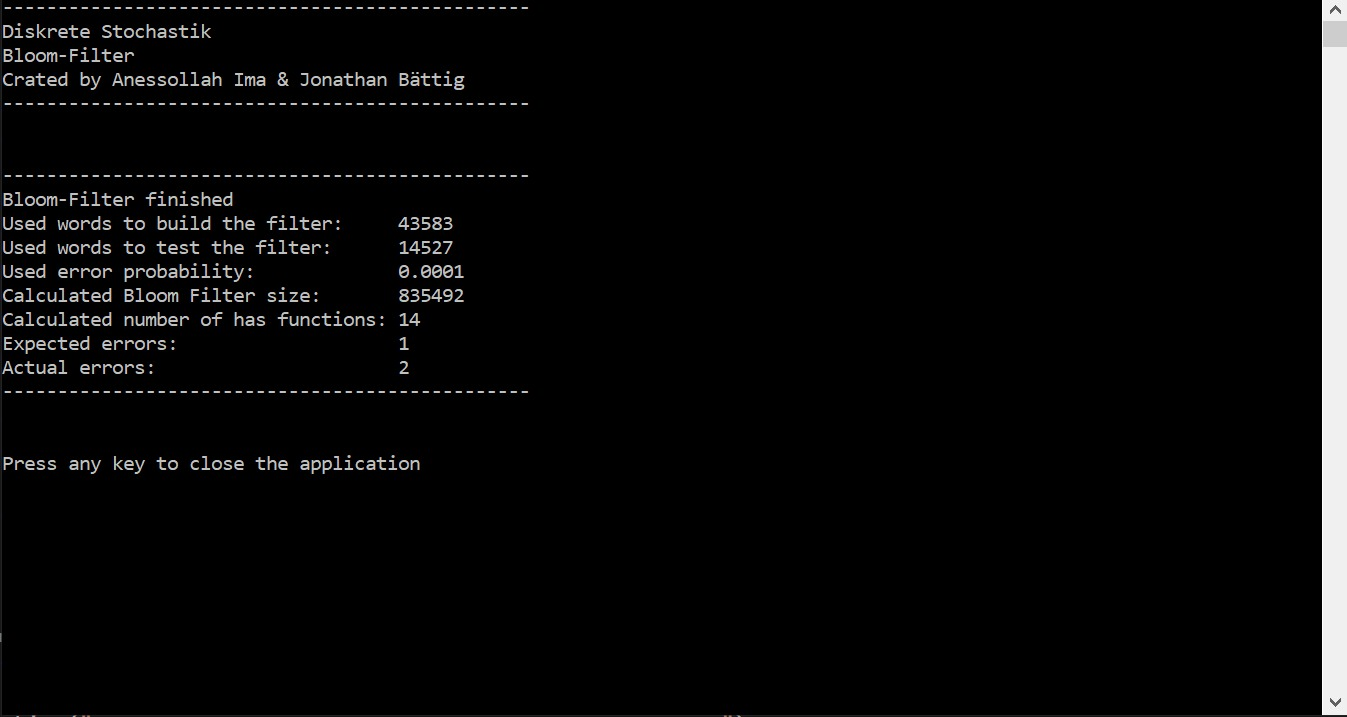
\includegraphics[width=\textwidth]{Program.jpg}

\begin{thebibliography}{9}
\bibitem{Wikipedia}Wikipedia (2005): Bloom filter [\url{https://en.wikipedia.org/wiki/Bloom\_filter}{https://en.wikipedia.org/wiki/Bloom\_filter}]
\bibitem{Youtube}Tech Dummies - Narendra L (2018): Bloom filter for System Design (YouTube) [\url{https://www.youtube.com/watch?v=Bay3X9PAX5k}]
\bibitem{TheMorpheusTutorials}The Morpheus Tutorials (2018): Bitcoin Tutorial \#34 - Bloom Filter (YouTube) [\url{https://www.youtube.com/watch?v=tURba0N50Cg}]
\bibitem{Testsite} Hurst, Thomas (2018): Bloom Filter Calculator [\url{https://hur.st/bloomfilter/}]
\end{thebibliography}

\end{document}
